%%%%%%%%%%%%%%%%%%%%%%%%%%
%%Preamble
%%%%%%%%%%%%%%%%%%%%%%%%%%
\documentclass[11pt, letterpaper, oneside]{article}

\usepackage[utf8]{inputenc}
\usepackage[T1]{fontenc}
\usepackage{graphicx}
\usepackage{pdfpages}
\usepackage{todonotes}
\usepackage{multirow}
\usepackage[a4paper, total={15.24cm, 25cm}]{geometry}
\usepackage{biblatex}
\addbibresource{Bibliography.bib}
\usepackage{float}
\usepackage{mathtools}
\usepackage{lscape}

%%%%%%%%%%%%%%%%%%%%%%%%%%%%%%%%%%%%%%%%%%%%%%%%%%%%%%%%%%%%%%%%%%%%
% Title page METADATA

%\thesistype{Master's Thesis} % Master's Thesis, Bachelor's Thesis, Semester Thesis, Group Project
\title{Eating up blue and green infrastructure: using remote sensing to identify backfill areas and characterize drivers of their distribution in Antananarivo}

\author{Carl Joseph}

\date{\today}
%\email{student@ethz.ch}

%\institute{Planning of Landscapes and Urban Systems (PLUS) \\[2pt]
%Environmental System's Sciences \\[2pt]
%ETH Zürich}

% Optionally, you can put in your own logo here
%\logo{\includegraphics[width=0.2\columnwidth]{figures/disco_logo_faded}}


% Optionally, keywords and categories of the work can be shown (on the Abstract page)
%\keywords{Keywords go here.}
%\categories{ACM categories go here.}

\renewcommand*\contentsname{Contents}


%%%%%%%%%%%%%%%%%%%%%%%%%%%%%%%%%%%%%%%%%%%%%%%%%%%%%%%%%%%%%%%%%%%%
%%%%%%%%%%%%%%%%%%%%%%%%%%
%%Document
%%%%%%%%%%%%%%%%%%%%%%%%%%
\begin{document}

\begin{titlepage}
\begin{figure}%[h]
    %\centering
    
\includegraphics{figures/eth_logo_black.eps}
\end{figure}
\maketitle

\begin{center}
\large
{Master's Thesis\\
\vspace{0.5cm}
Planning of Landscapes and Urban Systems (PLUS) \\[2pt]
Environmental System's Sciences \\[2pt]
ETH Zürich\\
\vspace{0.5cm}
Supervisor: Prof. Dr. Adrienne Grêt-Regamey\\
Co-Supervisors: Dr. Maarten Jan Van Strien, Dr. Nicolas Salliou}
\end{center}

\end{titlepage}


\addcontentsline{toc}{section}{Acknowledgements}
\section*{Acknowledgements}

\addcontentsline{toc}{section}{Abstract}
\section*{Abstract}

\addcontentsline{toc}{section}{Abbreviations}
\section*{Abbreviations}

\begin{description}
   \item[BGI]Blue and Green Infrastructure
   \item[ROI] Region Of Interest
   \item[Tana] Antananarivo
   \item[TD] Training Data
   
\end{description}

%\section*{Contents}
\tableofcontents

\section{Introduction}
flooding seasonality

grwowth o the city, urban sprawl and implications

nececcisy and controversy about backfills

definition and seasonality of backfils




\section{Methods}
\subsection{GIS tools and approach}
Description of GIS tools (GEE and ArcGis) that where used for the analyses and inclusion of a process chart, which shows the analyses steps f the agorithm in GEE.

\subsection{Study region}
The study region consists of the city of Antananarivo (Tana) and its surrounding Regions, also known as Greater Antananarivo. Tana is the capital of Madagascar, a city which grew on inhabited hills surrounded by a flood prone plain, which is used for agriculture (e.g. rice cultivation). The climate in Tana Is warm and temperate, with a dry season in winter and a rainy season in summer. Typically, there can be seasonal floods due o the high precipitation in the rainy season.  
As a Region of interest (ROI) for my analysis I chose the buffered boundaries of Greater Tana  as also used by Dupuy et al \cite{Dupuy.2020b}. Further, the region was restricted to the low plains, since these are the main areas for cultivation of rice and other irrigated crops. areas within the ROI at an elevation below 1260 m.a.s.l. and with a slope smaller than 10° where chosen as Study region. 
In a later step I discarded a part of the ramainin area to the north west of Tana due to suspected misclassifications. This was done along the watershed boundary in order to keep areas that are upstream from the city in the study region. Image X shows the final study region that was chosen, and the buffered outline of Greater Tana.

\subsection{Satellite Images}

\subsubsection{Image collection}
To create an image time-series on a yearly bases it was necessary to find at least one satellite image per year. These images should be from a similar time during the year to have similar atmospheric and vegetation conditions. Due to backfills occurring in the dry season the images where collected outside of this time-period. The idea being to capture most backfills that took place in one year by using satellite images outside of the season when backfills mainly take place. I tried different appoaches of image acquisition. First looking for single images in May or June after the rainy season. This proved to be difficult due to there often being high cloud cover over Tana, which meant that in some cases the first cloud free image (over the city) was from August or September, thus negating the idea of taking images outside of the dry season. The problem of high cloud cover lead to the idea of using image-composites, meaning to combine the data of several images, o a certain time period. Doing this all images originating in a certain time period could  be filtered for the percentage of cloud cover and  masked for clouds to exclude clouy pixels .The remaining images and pixels where then combined to one by taking the mean value per pixel.
\subsubsection{Pre-processing}
The collected images were further processed, for the later analysis. For this they were clipped to fit the size of the ROI, which contains most rice fields and other BGI. This has the advantage of excluding areas that are not directly relevant to the research question from the analysis and of limiting the amount o data that is created and processed. As a further step the band values of the images where used to calculate different indices, such as the Bare Soil Index (BSI), and ratios between diferent bands to use for the classification. Indices and band ratios can be beneficial for classification purposes, because they are less susceptible to changes due to atmospheric conditions or lighting differences than the band values themselves. This is especially the case for the bands containing reflectance information for wavelength in the visible light rage. A digital elevation model (DEM) was used to also add elevation and calculated slope data to the images for classification. The image bands that where used for the classification are listed in table \ref{tab:bandratios}.

\begin{landscape}
\begin{table}
\caption{List of band indices and ratios that were calculated from image bands and added to the image for later use in classification. The Band names in the formulas represent Landsat 8 bands.}
\centering
\bgroup%start group
\def\arraystretch{2}%define cell height (for formula visibility)
\begin{tabular}{c c c}
  \hline
 Index/ Band ratio & Formula & References  \\ 
  \hline
Atmospherically Resistant Vegetation Index (ARVI) & \(\frac{(NIR-(2\cdot RED)+BLUE)}{(NIR+(2 \cdot RED)+BLUE}\) & \cite{Yuvaraj.2022}\cite{Kaufman.1992}\\
Bare Soil Index (BSI)& \(\frac{((RED+SWIR2)-(NIR+BLUE))}{((RED+SWIR2)+(NIR+BLUE))}\)& \cite{Diek.2017}\\
Colour Index (CI) & \(\frac{(RED-GREEN)}{(RED+GREEN)}\) &\cite{Yuvaraj.2022}\\
Normalized Diference Built up Index (NDBI) & \(\frac{(SWIR1-NIR)}{(SWIR1+NIR)}\) & \cite{Zha.2003}\\
Normalized Difference Vegetation Index (NDVI)& \(\frac{(NIR-RED)}{(NIR+RED)}\) &\\
Normalized Difference Water Index (NDWI)& \(\frac{(GREEN-NIR)}{(GREEN+NIR)}\) & \cite{McFEETERS.1996}\\
Redness Index (RI)& \(\frac{(RED^2)}{(GREEN^2)}\) & \cite{Yuvaraj.2022}\\
%Soil Composition Index (SCI)& (SWIR1-NIR)/(SWIR1+NIR) \cite{AlKhaier.2003}&\\
Ratio 4/3 & \(\frac{RED}{GREEN}\) & \cite{Mwaniki.2015}\\
Ratio 5/7 & \(\frac{NIR}{SWIR2}\) & \cite{NgoThi.2019}\\
Ratio 6/2 & \(\frac{SWIR1}{BLUE}\) & \cite{Mwaniki.2015}\\
Ratio 7/3 & \(\frac{SWIR2}{RED}\) & \cite{Mwaniki.2015}\\

            
   \hline
\end{tabular}
\egroup%end group
\label{tab:bandratios}
\end{table}
\end{landscape}

\subsection{Training Data}

\subsection{Classification}

\subsection{Validation}

\subsubsection{Classification algorithm}
To use as much data as possible for training and to have a good estimation of accuracy, I chose to employ a k-fold cross-validation. If the large sample parameter is met it is best to do one run with ten folds \cite{Wong.2020}.
\subsubsection{Backfill time-series}

\subsection{Data analysis}

\subsubsection{Backfill time-series}

\subsubsection{Logistic regression} 

\newpage
\section{Results}

\subsection{Backfill time-series}
A time-series was created by masking classified backfills in one year with the backfills in the years before, resulting in a yearly increase which was then used to calculate the area. The red circles and blue triangles in figure \ref{fig:areakm2} show the area calculation with all available training data and the down-sampled training data respectively. Mainly for the years 2014, 2017 and 2022 there is considerable overestimation of backfill area increase comparing the results of the down-sampled data to using all data (17 - 27\% decrease). Other than that the values are similar, those calculated using all TD being slightly lower (4 - 12\% decrease). 
In the further analysis the down-sampled TD was used for all calculations. Thus hoping to avoid any biases due to the over-fitting of abundant classes like rice in the supervised classification.
The evolution of backfill area increase per year did not show a clear trend. Over the observed time-period there is some degree of variance (Y), but most values are in the same ballpark as the mean of 0.72 $km^2yr^{-1}$.
The values for the following three years stand out compared to the others. 2016 (0.15 $km^2$) and 2021 (0.29 $km^2$) show a low backfill area increase, whereas the value for 2017 (1.7 $km^2$) is the highest.

\begin{figure}[H]
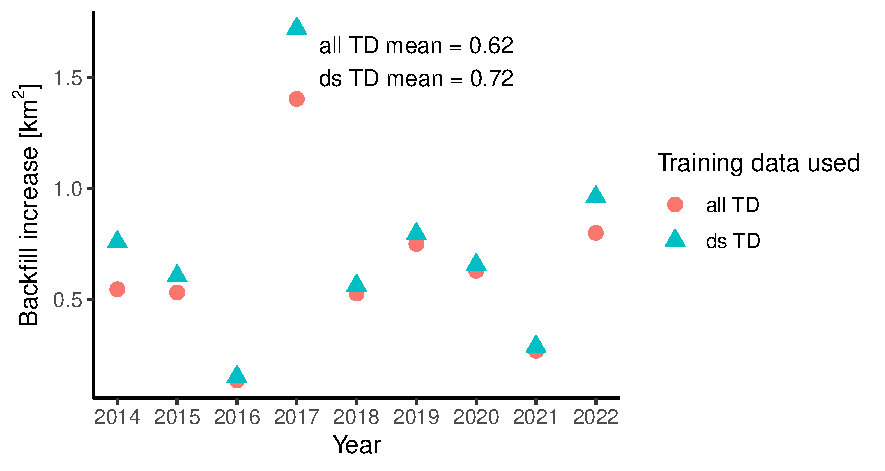
\includegraphics[width = 15cm]{figures/Backfill area increase km 2.pdf}
\caption{Yearly backfill area increase [$km^2yr^{-1} $] in the study region around Antananarivo. The years are indicative of the rainy season (December - March), to which each classified image composite relates. The area values represent the increase in backfill area since the rainy season in the year before. Red dots show the results when all TD is used and blue triangles when only the downsampled (ds) TD-set is used.}
\label{fig:areakm2}
\end{figure}

Figure \ref{fig:BFtypo} indicates that most areas classified as backfill are small, spanning 900 $m^2$, meaning they consist of one pixel of the classified image (30x30m). This shows that also smaller areas have a considerable impact on the overall backfill area and yearly increase.

\begin{figure}[H]
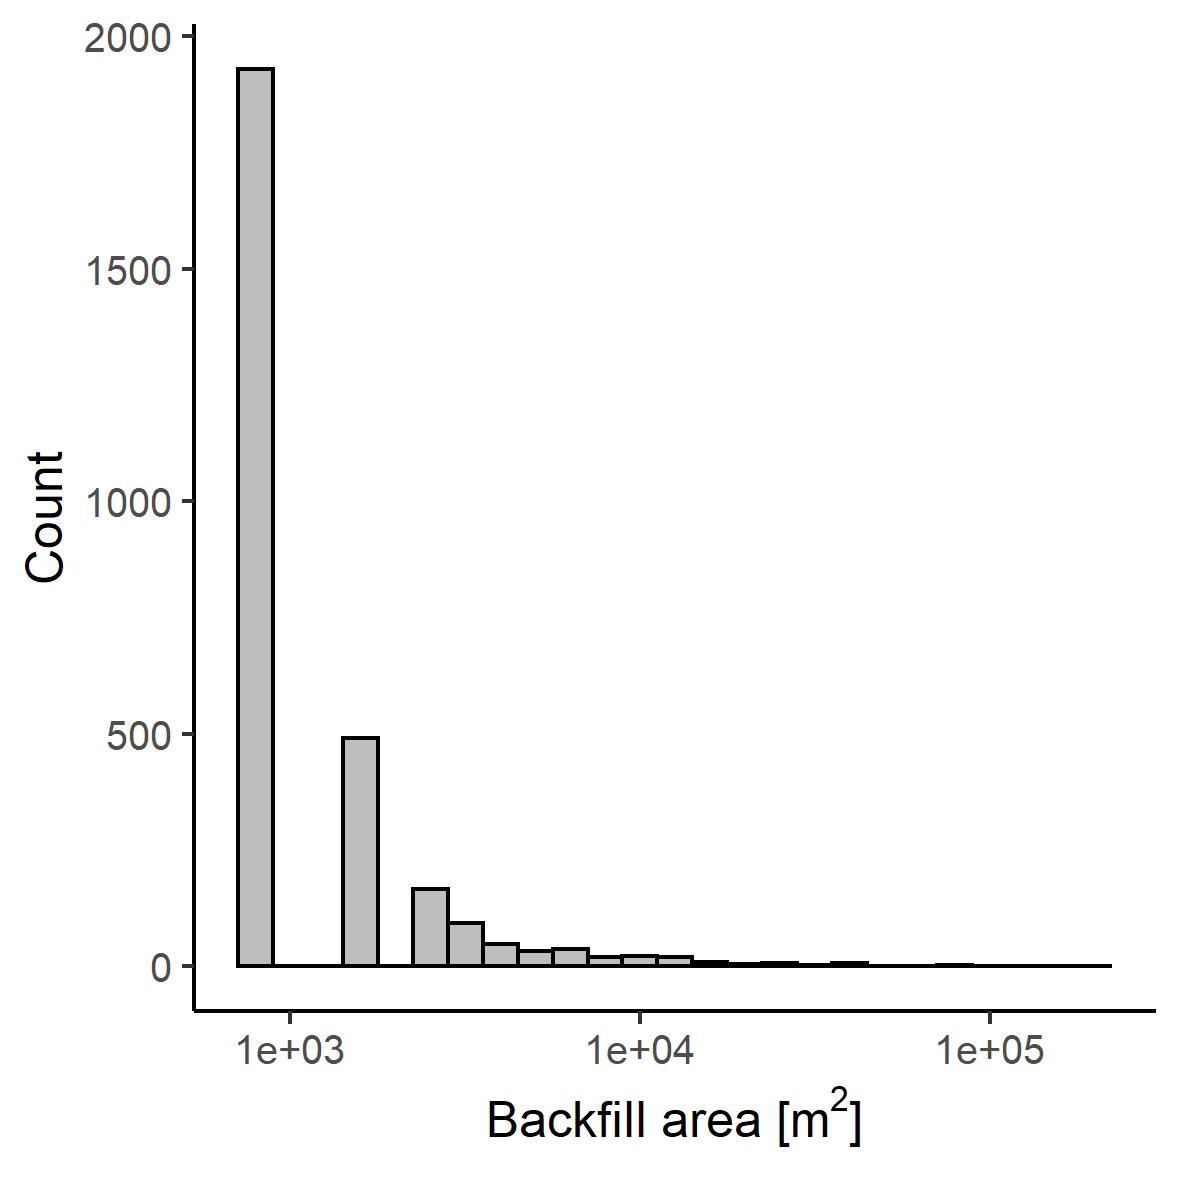
\includegraphics[width = 10cm]{figures/Backfill typology sizes.jpeg}
\caption{Size distribution among the areas classified as backfill. A histogram of the frequency of backfills per area [$m^2$] of the respective site.}
\label{fig:BFtypo}
\end{figure}

\subsection{Logistic regression} 
Logistic regression was employed to analyse the influence of different independent variables (table \ref{tab:logreg_allyrs}) on backfills that occured a year later. The independent variables of this regression analysis consist of continuous numerical data of slope, elevation and distances to other landcover classes (in the year before), as well as categorical factors indicating the classification of a pixel in the previous year.  
Figure \ref{fig:logibox} shows boxplots for two of these variables comparing backfills (yearly increase) to the control dataset, which was randomly chosen from pixels of other lancover classes to fit the size of the backfill data. Backfills are often associated with a closer proximity to existing backfills from previous years than other landcover classes.
This is consistent with the results of the regression analysis (Table \ref{tab:logreg_allyrs}). The regression model does not fit the data very well, with an R$^2$ (Mc Fadden) of 0.11. This indicates that the model does not fully explain  the distribution and occurrence of new backfills and there could be other, unknown factors having a strong influence. Holding all other variables constant, the odds for new backfill decreased by 0.12\% (95\% CI [-0.0013, -0.0011]) for a unit increase (m) in distance to already existing backfills. A classification as rice was found to decrease the odds for new backfill a year later by 55\% (95\% CI [-0.6, -0.4916]). Similarly, for a classification as wetland or built-up area the model shows a probability decrease of 58\% (95\% CI [-0.6338, -0.5143]) and 66\% (95\% CI [-0.7068, -0.6091]) respectively for the occurrence of new backfills a year later. Each estimate is given under the assumption that all other variables are constant. Other than for slope, the variables all have significant p-values far below 0.05.

\begin{figure}[H]
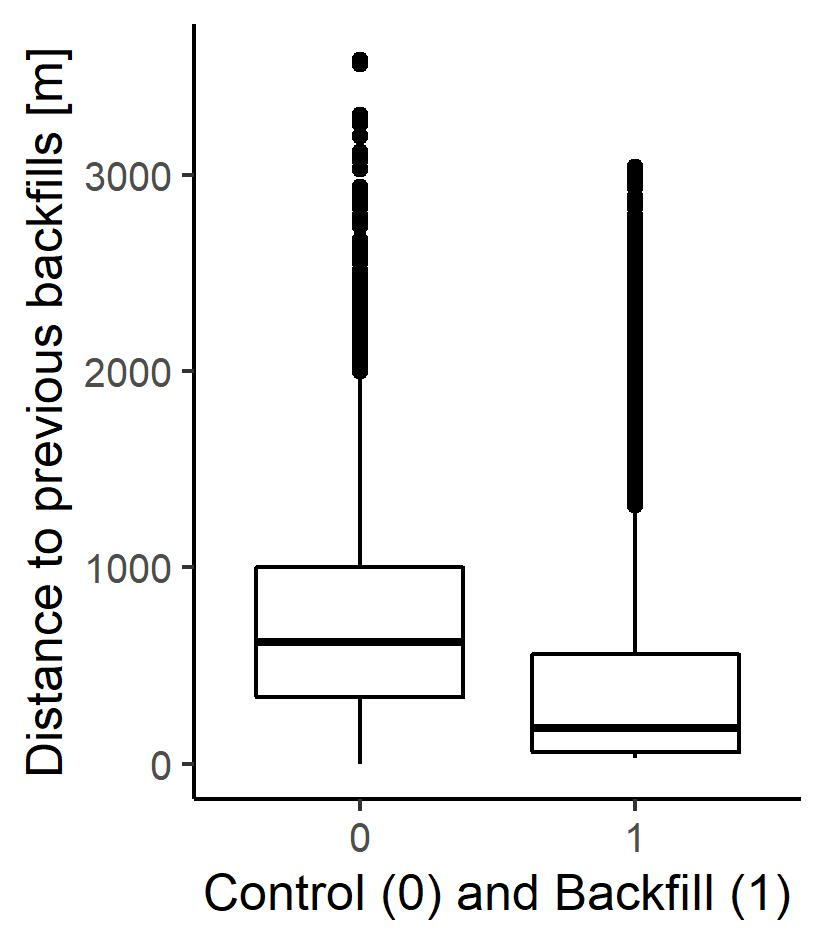
\includegraphics[width = 7 cm]{figures/boxplot backfill logi.jpg}
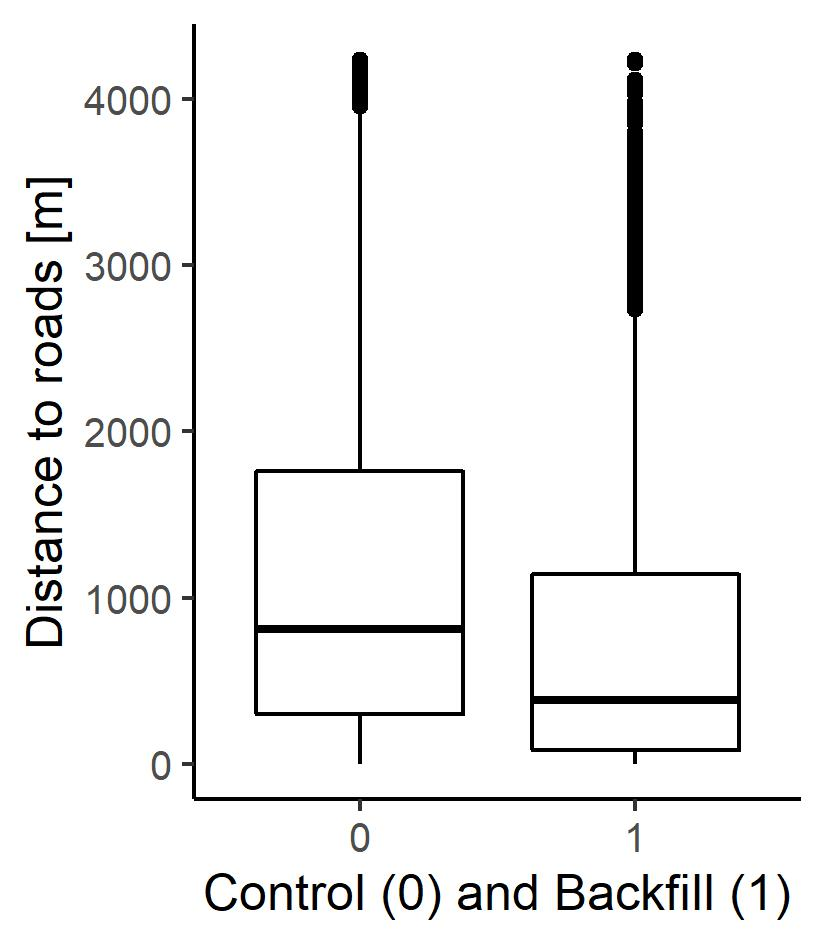
\includegraphics[width = 7 cm]{figures/boxplot roads logi.jpg}
\caption{Comparison of the yearly backfill increments and control with respect to the distance [m] to backfills in the previous year and roads.}
\label{fig:logibox}
\end{figure}


\begin{table}[H]
\caption{Summary of the logistic regression. For all independent variables used, the odds ratio (OR), lower and upper boundaries (Low, Up) of the 95\% confidence interval, variable importance (VI) and the p - value (P) are given. The overall analysis has a pseudo R$^2$ (Mc Fadden) of 0.11.}
\centering
\begin{tabular}{c c c c c c c}
  \hline
 Unit & Variables & OR & Low & Up & VI & P \\ 
  \hline
m.a.s.l. [m] &  Elevation & 1.016 & 1.0053 & 1.0268 & 2.9323 & 0.00336 \\ 
Slope [°] & Slope & 1.0057 & 0.984 & 1.028 & 0.5121 & 0.609 \\ 
\hline
 \multirow{8}{3cm}{Distance [m] to land cover in the previous year} 
                    & Roads  & 0.9998 & 0.9998 & 0.9999 & 6.8411 & 7.86e-12 \\ 
                    & \textbf{Backfill}  & 0.9988 & 0.9987 & 0.9989 & \textbf{25.9418} & 2.25e-148 \\ 
                    & Built-up  & 0.9995 & 0.9992 & 0.9998 & 3.2728 & 0.00106 \\ 
                    & Industrial  & 1.0003 & 1.0002 & 1.0004 & 4.5562 & 5.21e-06 \\ 
                    & Waterbodies & 0.9995 & 0.9994 & 0.9997 & 8.235 & 1.8e-16 \\ 
                    & Wetland & 0.9989 & 0.9984 & 0.9993 & 4.8607 & 1.17e-06 \\ 
                    & Rice & 0.9981 & 0.9973 & 0.999 & 4.4006 & 1.08e-05\\ 
                    & Watercress & 0.9995 & 0.9992 & 0.9998 & 3.3832 & 0.000716 \\ 
                    \hline
\multirow{6}{3cm}{Previous year classification (factor of 0/1)} 
            & Rice & 0.4509 & 0.4 & 0.5084 & 13.0269 & 8.61e-39\\ 
            & Watercress & 0.4837 & 0.4148 & 0.5641 & 9.2604 & 2.04e-20 \\ 
            & Wetland & 0.4217 & 0.3662 & 0.4857 & 11.9852 & 4.25e-33\\ 
            & Waterbodies & 0.3731 & 0.3059 & 0.4551 & 9.7285 & 2.28e-22 \\ 
            & Industrial & 0.703 & 0.5758 & 0.8583 & 3.4607 & 0.000539  \\ 
            & Built-up & 0.3385 & 0.2932 & 0.3909 & 14.7626 & 2.55e-49 \\ 
            
   \hline
\end{tabular}

\label{tab:logreg_allyrs}
\end{table}

Running the regression model separately for every year in the time-series shows a considerable difference in model fit over the years (figure \ref{fig:logitimeseries}). Supporting the overall analyses, there is a significant decrease in backfill probability with increasing distance to already existing backfills for all years. In most years the odds ratio of distance to roads also shows a decrease of backfill probability with increasing distance, though it is only significant for four years. 

\begin{figure}[H]
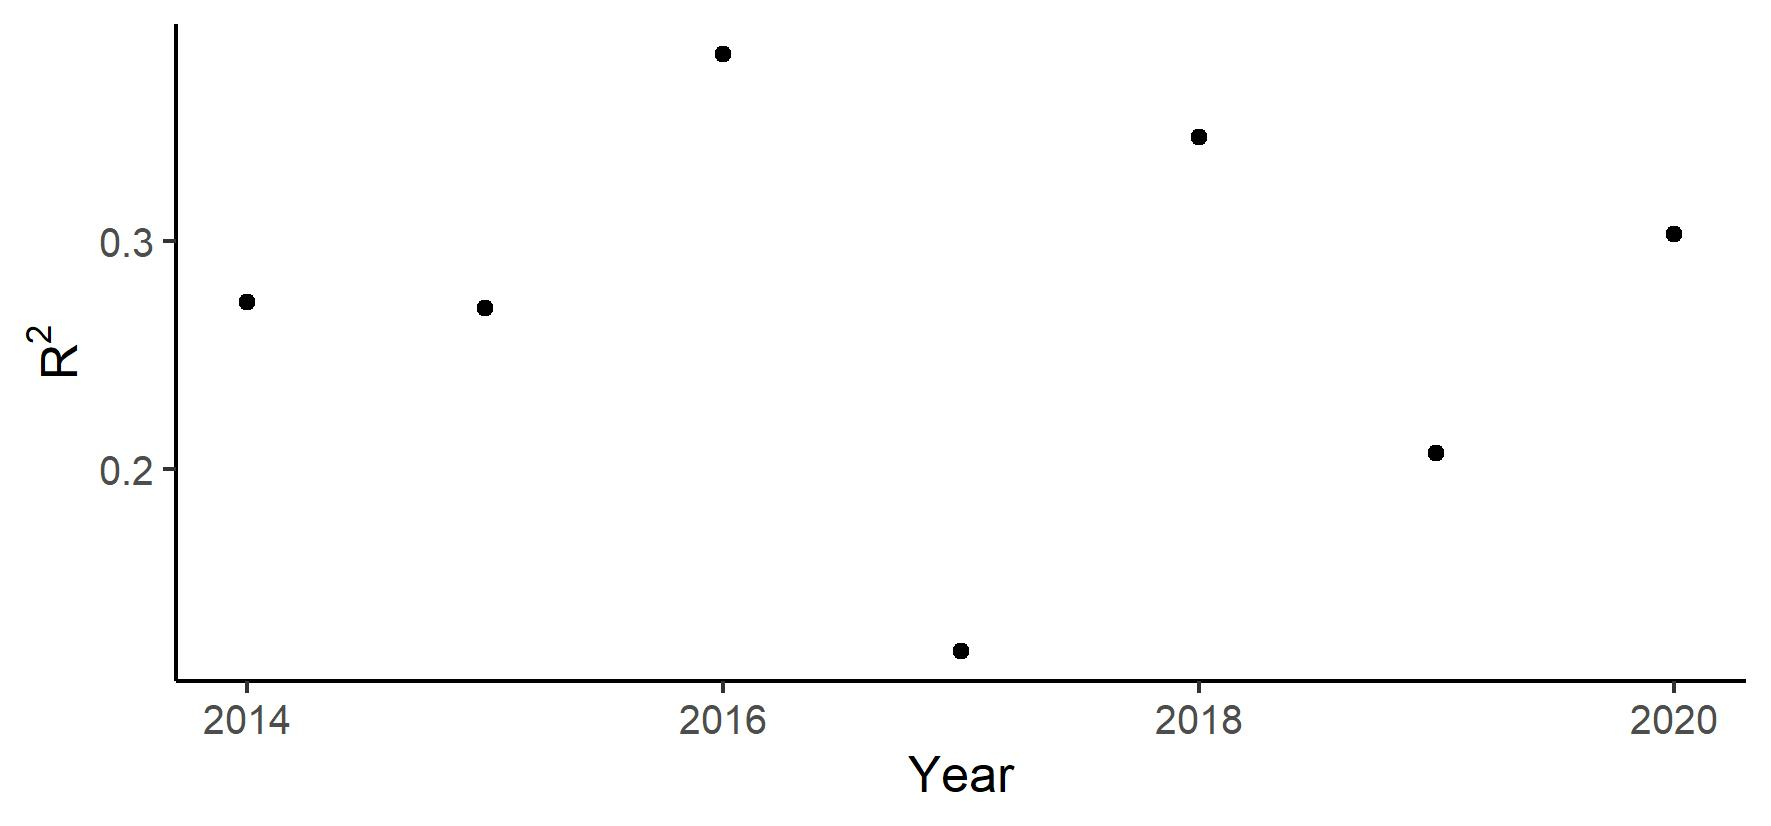
\includegraphics[width = 15 cm]{figures/logreg_year_Rsq.jpeg}
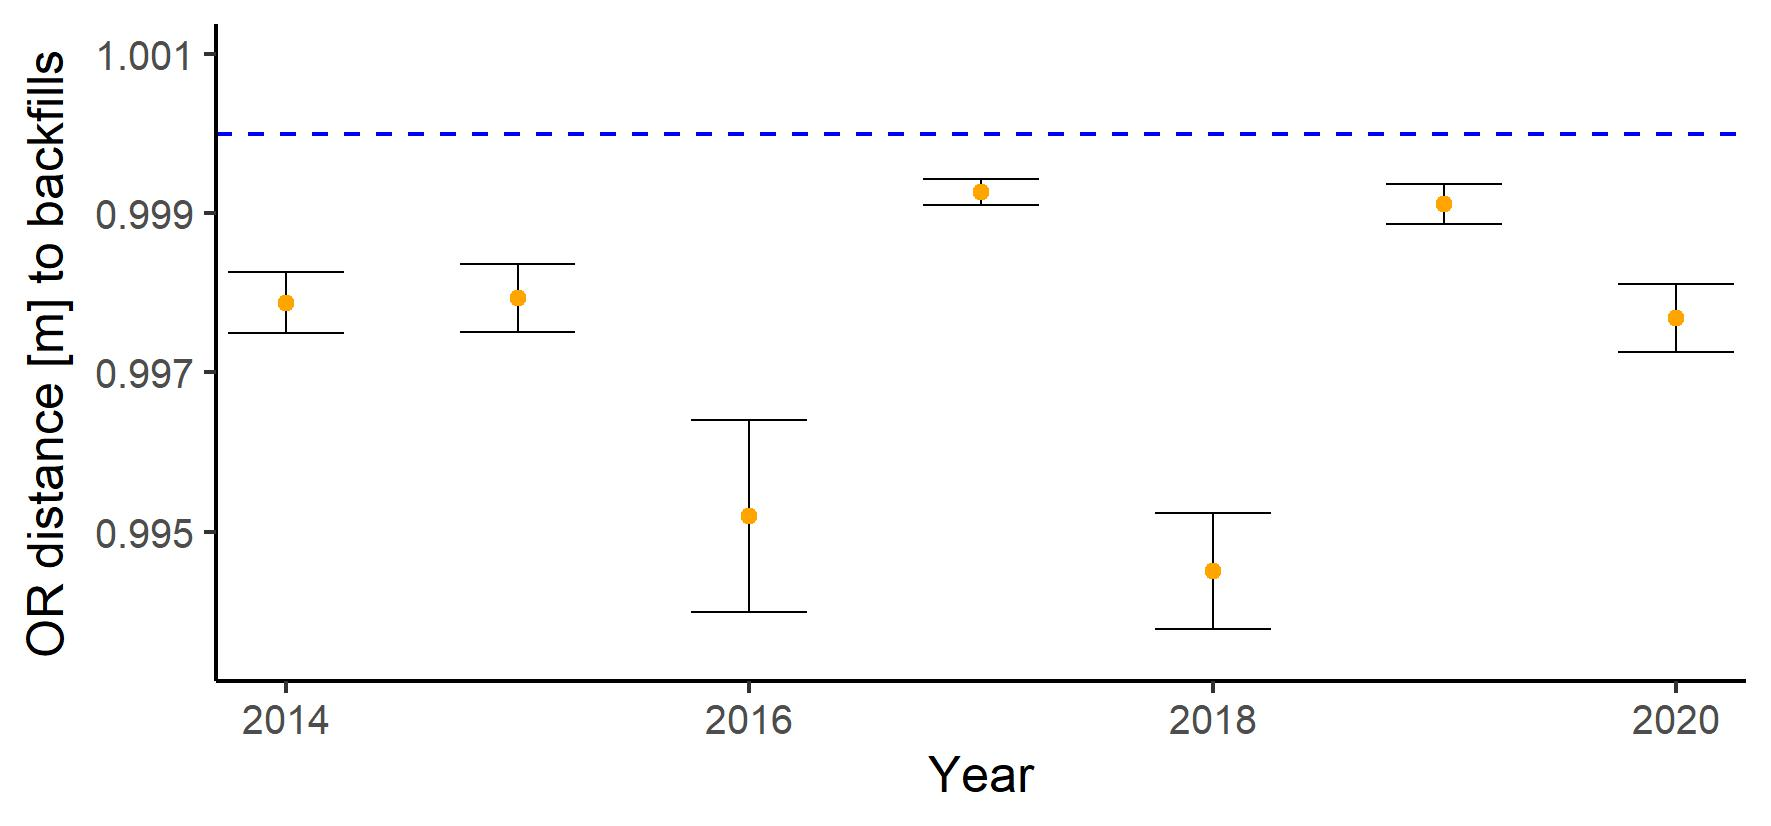
\includegraphics[width = 15 cm]{figures/logreg_year_BFdist.jpeg}
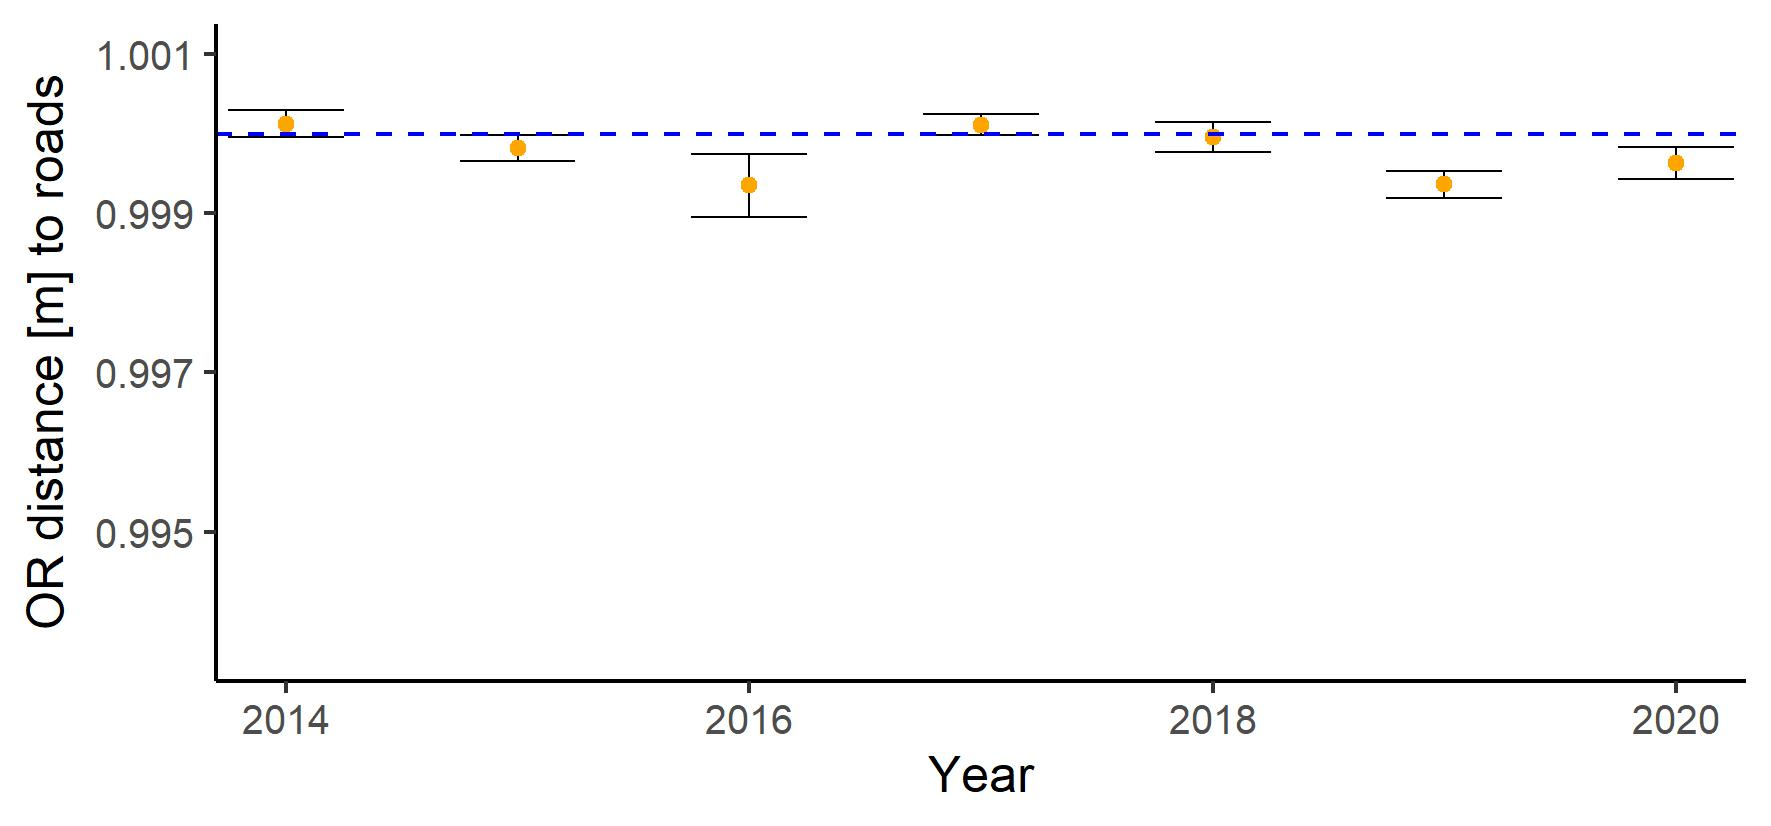
\includegraphics[width = 15 cm]{figures/logreg_year_Roadist.jpeg}
\caption{Overall R$^2$ (Mc Fadden) and odds ratios (OR) for the two variables distance to roads [m] and distance to backfills [m] of the previous year for the logistic regression when run for each year separately. The error bars show the 95\% confidence interval of the odds ratio.}
\label{fig:logitimeseries}
\end{figure}

\newpage
\section{Discussion}

\subsection{Backfill time-series}
The high value for 2016 might be explained by the construction of several new roads through the lower lands of Tana, requiring backfill for stabilization. also one of the largest backfilled areas in my study region shows considerable growth in this year

In January of 2014, Hery Rajaonarimampianina was sworn in as president following the elections.
In January of 2019 Andry Rajoelina won the presidential election. In both cases the backfill increase data shows a small dip in the year after and a stronger dip two years after. This might hint at an impact of new legislation (or plans for it) in the beginning of both presidential periods. In both cases this was subsequently followed by a relatively high value of yearly backfill increase, especially for the 2017 value. (https://www.bbc.com/news/world-africa-13864364 , 08.08.2022)

Comparison to other landcover changes

\subsection{Logistic regression} 

\section{Conclusion}

\addcontentsline{toc}{section}{Bibliography}
\section*{Bibliography}
\printbibliography

\end{document}
